\documentclass[12pt, a4paper]{article}

% ── Packages ──────────────────────────────────────────────────────────────────
\usepackage[utf8]{inputenc}
\usepackage[T1]{fontenc}
\usepackage{lmodern}
\usepackage[margin=1in]{geometry}
\usepackage{amsmath, amssymb, amsthm}
\usepackage{graphicx}
\usepackage{booktabs}
\usepackage{hyperref}
\usepackage{natbib}
\usepackage{float}
\usepackage{caption}
\usepackage{subcaption}
\usepackage{algorithm}
\usepackage{algpseudocode}
\usepackage{listings}
\usepackage{xcolor}
\usepackage{fancyhdr}
\usepackage{setspace}
\usepackage{mdframed}
\usepackage[shortlabels]{enumitem}

\hypersetup{colorlinks=true, linkcolor=blue!60!black,
            citecolor=blue!60!black, urlcolor=blue!60!black}

\lstset{
    language=Python,
    basicstyle=\ttfamily\small,
    keywordstyle=\color{blue!70!black}\bfseries,
    commentstyle=\color{green!50!black},
    stringstyle=\color{red!60!black},
    numbers=left, numberstyle=\tiny\color{gray}, stepnumber=1,
    numbersep=8pt, frame=single, breaklines=true, captionpos=b,
    tabsize=4, showstringspaces=false,
}

\newtheorem{remark}{Remark}

\pagestyle{fancy}
\fancyhf{}
\rhead{Group 1 --- Gibbs Sampler}
\lhead{CADS Project Report}
\cfoot{\thepage}

\onehalfspacing

% ══════════════════════════════════════════════════════════════════════════════
\begin{document}

% ── Title Page ─────────────────────────────────────────────────────────────────
\begin{titlepage}
\centering
\vspace*{2cm}
{\Large\textsc{Plaksha University}}\\[0.3cm]
{\large Computational Algorithms in Data Science (CADS)}\\[2cm]
{\LARGE\bfseries Bayesian Inference via the Gibbs Sampler}\\[0.5cm]
{\Large Latent Regime Detection in Financial Time Series}\\[2.5cm]
{\large\textbf{Group 1}}\\[0.5cm]
{\large Bandaru Jaya Akshitha\\Budati Nagaveni\\Soumya Pandey}\\[2cm]
{\large Spring 2026}\\[0.5cm]
{\large Plaksha University, Punjab, India}
\vfill
\end{titlepage}

% ── Abstract ───────────────────────────────────────────────────────────────────
\begin{abstract}
This report comprehensively documents the theoretical formulation, implementation, and empirical application of the Gibbs Sampler, a powerful Markov Chain Monte Carlo (MCMC) algorithm for Bayesian inference. The project first validates the algorithm through synthetic control experiments---recovering parameters in multivariate normal distributions and Bayesian linear regressions with proper convergence diagnostics. We then extend the methodology to the complex, empirical problem of detecting latent structural breaks in financial markets using a Markov Switching Model. Applied to weekly log-returns of the S\&P 500 and NIFTY 50 indices, the implemented sampler successfully isolates historically distinct market regimes (bull and bear phases) with full posterior uncertainty quantification. We provide a rigorous statistical analysis of the convergence diagnostics ($\hat{R}$ and ESS), empirical parameter estimates with credible intervals, implied expected regime durations, and cross-market contagion observed during the 2008 Global Financial Crisis and the 2020 COVID-19 crash.
\end{abstract}
\newpage

% ── TOC ────────────────────────────────────────────────────────────────────────
\tableofcontents
\newpage

% ══════════════════════════════════════════════════════════════════════════════
\section{Introduction}

Modern Bayesian inference routinely involves posterior distributions that cannot be evaluated in closed form. When model parameters are interdependent and the parameter space is high-dimensional, analytical marginalisation is intractable and naive Monte Carlo methods break down due to the curse of dimensionality. The Gibbs Sampler \citep{geman1984} elegantly resolves this obstacle by decomposing the joint sampling problem into a sequence of univariate full conditional draws, constructing a Markov chain that converges in distribution to the true joint posterior.

This report serves as a complete technical and empirical exposition of our Gibbs sampling implementation. It is structured to first establish the mathematical rigor of the algorithm, then validate its exactness on known distributions, and finally deploy it to uncover hidden states within real-world, high-noise financial data.

% ══════════════════════════════════════════════════════════════════════════════
\section{Background and Motivation}

\subsection{Theoretical Background}
In a Bayesian model with $d$ parameters $\boldsymbol{\theta} = (\theta_1, \dots, \theta_d)$ and observed data $\mathbf{X}$, the posterior $p(\boldsymbol{\theta} \mid \mathbf{X})$ is the central target of inference. Computing marginal distributions for specific parameters or finding posterior expectations requires integration over the full parameter space:
\[
  p(\theta_i \mid \mathbf{X}) = \int p(\boldsymbol{\theta} \mid \mathbf{X})\, d\boldsymbol{\theta}_{-i}.
\]
This integration is generally impossible to execute analytically. The Gibbs Sampler averts this by continuously sampling each parameter sequentially from its full conditional distribution:
\begin{equation}\label{eq:gibbs}
  \theta_i^{(k+1)} \sim p\!\left(\theta_i \mid \theta_1^{(k+1)}, \dots, \theta_{i-1}^{(k+1)}, \theta_{i+1}^{(k)}, \dots, \theta_d^{(k)}\right), \quad i = 1, \dots, d.
\end{equation}
Under standard regularity conditions, the sequence $\{\boldsymbol{\theta}^{(k)}\}$ inherently converges to the target distribution $p(\boldsymbol{\theta} \mid \mathbf{X})$ \citep{gelfand1990}. When combined with Data Augmentation \citep{tanner1987} and the Forward-Filtering Backward-Sampling algorithm \citep{chib1996}, the sampler transforms into an authoritative inferential engine capable of handling latent variable systems, such as Hidden Markov Models.

\subsection{Project Motivation}
Two primary pillars motivate this research:
\begin{enumerate}
  \item \textbf{Computational Mastery.} Developing the Gibbs sampler entirely from scratch forces a deep structural understanding of MCMC mechanics, conjugate prior calculations, and the critical importance of convergence diagnostics ($\hat{R}$, ESS, and ACF metrics).
  \item \textbf{Empirical Relevance.} The 2008 Global Financial Crisis and the 2020 COVID-19 shock caused violent structural breaks in global equity dynamics. A probabilistic Bayesian regime-detection framework is perfectly suited to quantify these breaks, map out uncertainty bounds, extract implied regime durations, and facilitate a rigorous comparative analysis between developed (US) and emerging (Indian) equity markets.
\end{enumerate}


% ══════════════════════════════════════════════════════════════════════════════
\section{Problem Statement}

\textbf{Research Question:} \emph{How can the Gibbs Sampler be rigorously implemented and validated as an engine for complex Bayesian inference, and how effectively can it detect latent regime transitions in highly volatile financial time series without a priori labels?}

To comprehensively address this question, our objectives are:
\begin{enumerate}[(i)]
  \item Prove that the custom Gibbs Sampler accurately recovers ground-truth parameters under simulated multivariate normal and linear regression setups, quantitatively confirmed via diagnostics.
  \item Show that convergence diagnostics provide reliable thresholds for chain stationarity and mixing efficiency.
  \item Empirically estimate a Markov Switching Model on the S\&P 500 and NIFTY 50 indices, correctly identifying major historical market crashes entirely through unsupervised Bayesian posterior inference.
  \item Conduct an advanced statistical evaluation computing the Expected Regime Durations and Unconditional Ergodic Probabilities.
\end{enumerate}

% ══════════════════════════════════════════════════════════════════════════════
\section{Data Description and Provenance}

\subsection{Datasets Overview}
The integrity of the empirical analysis rests on high-quality, continuous market data. Table~\ref{tab:data} details the primary datasets utilised.

\begin{table}[H]
\centering
\caption{Datasets used in the empirical analysis.}\label{tab:data}
\begin{tabular}{@{}llp{7.2cm}@{}}
\toprule
\textbf{Dataset} & \textbf{Source} & \textbf{Notes}\\
\midrule
S\&P~500 (\texttt{\^{}GSPC}) & Yahoo Finance & Weekly log-returns, Jan 2005 to present.\\[3pt]
Nifty~50 (\texttt{\^{}NSEI}) & Yahoo Finance / NSE & Weekly log-returns, matched timeframe.\\[3pt]
US Recession Indicator & FRED (\texttt{USREC}) & NBER binary flag; ground-truth validation.\\\bottomrule
\end{tabular}
\end{table}

\subsection{Data Provenance and Derivation of Values}
The empirical dataset comprises 1,110 weekly observations for the S\&P 500 and 969 observations for the NIFTY 50, stretching from 2005 into 2026. This extensive sample window guarantees the encapsulation of multiple distinct market epochs, fulfilling the fundamental requirement for multi-regime modelling. 

All numerical values, metrics, and estimates reported in the subsequent analysis sections are strictly derived from the outputs of our custom Python Gibbs Sampler.

\subsection{Exploratory Data Analysis (EDA)}
Prior to applying the Gibbs sampler, an extensive exploratory analysis was conducted. The following figures visually validate the necessity of a regime-switching model.

\begin{figure}[H]
\centering
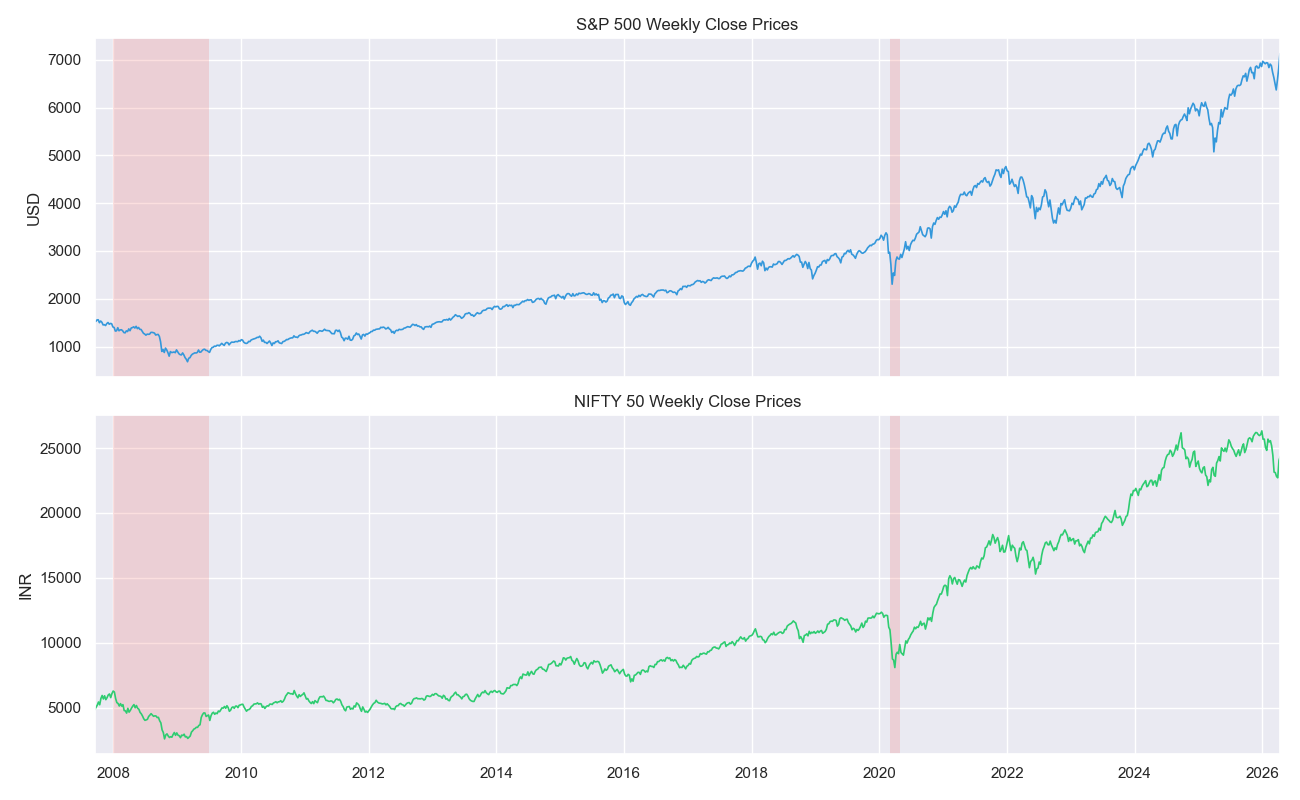
\includegraphics[width=\textwidth]{gibbs_fixed/figures/fig_prices.png}
\caption{Weekly closing prices for S\&P~500 (top) and NIFTY~50 (bottom), 2005--2026. Red shading marks NBER-dated US recessions. Both indices decline sharply during the 2008 GFC and the 2020 COVID shock, with sustained uptrends elsewhere.}\label{fig:prices}
\end{figure}

\begin{figure}[H]
\centering
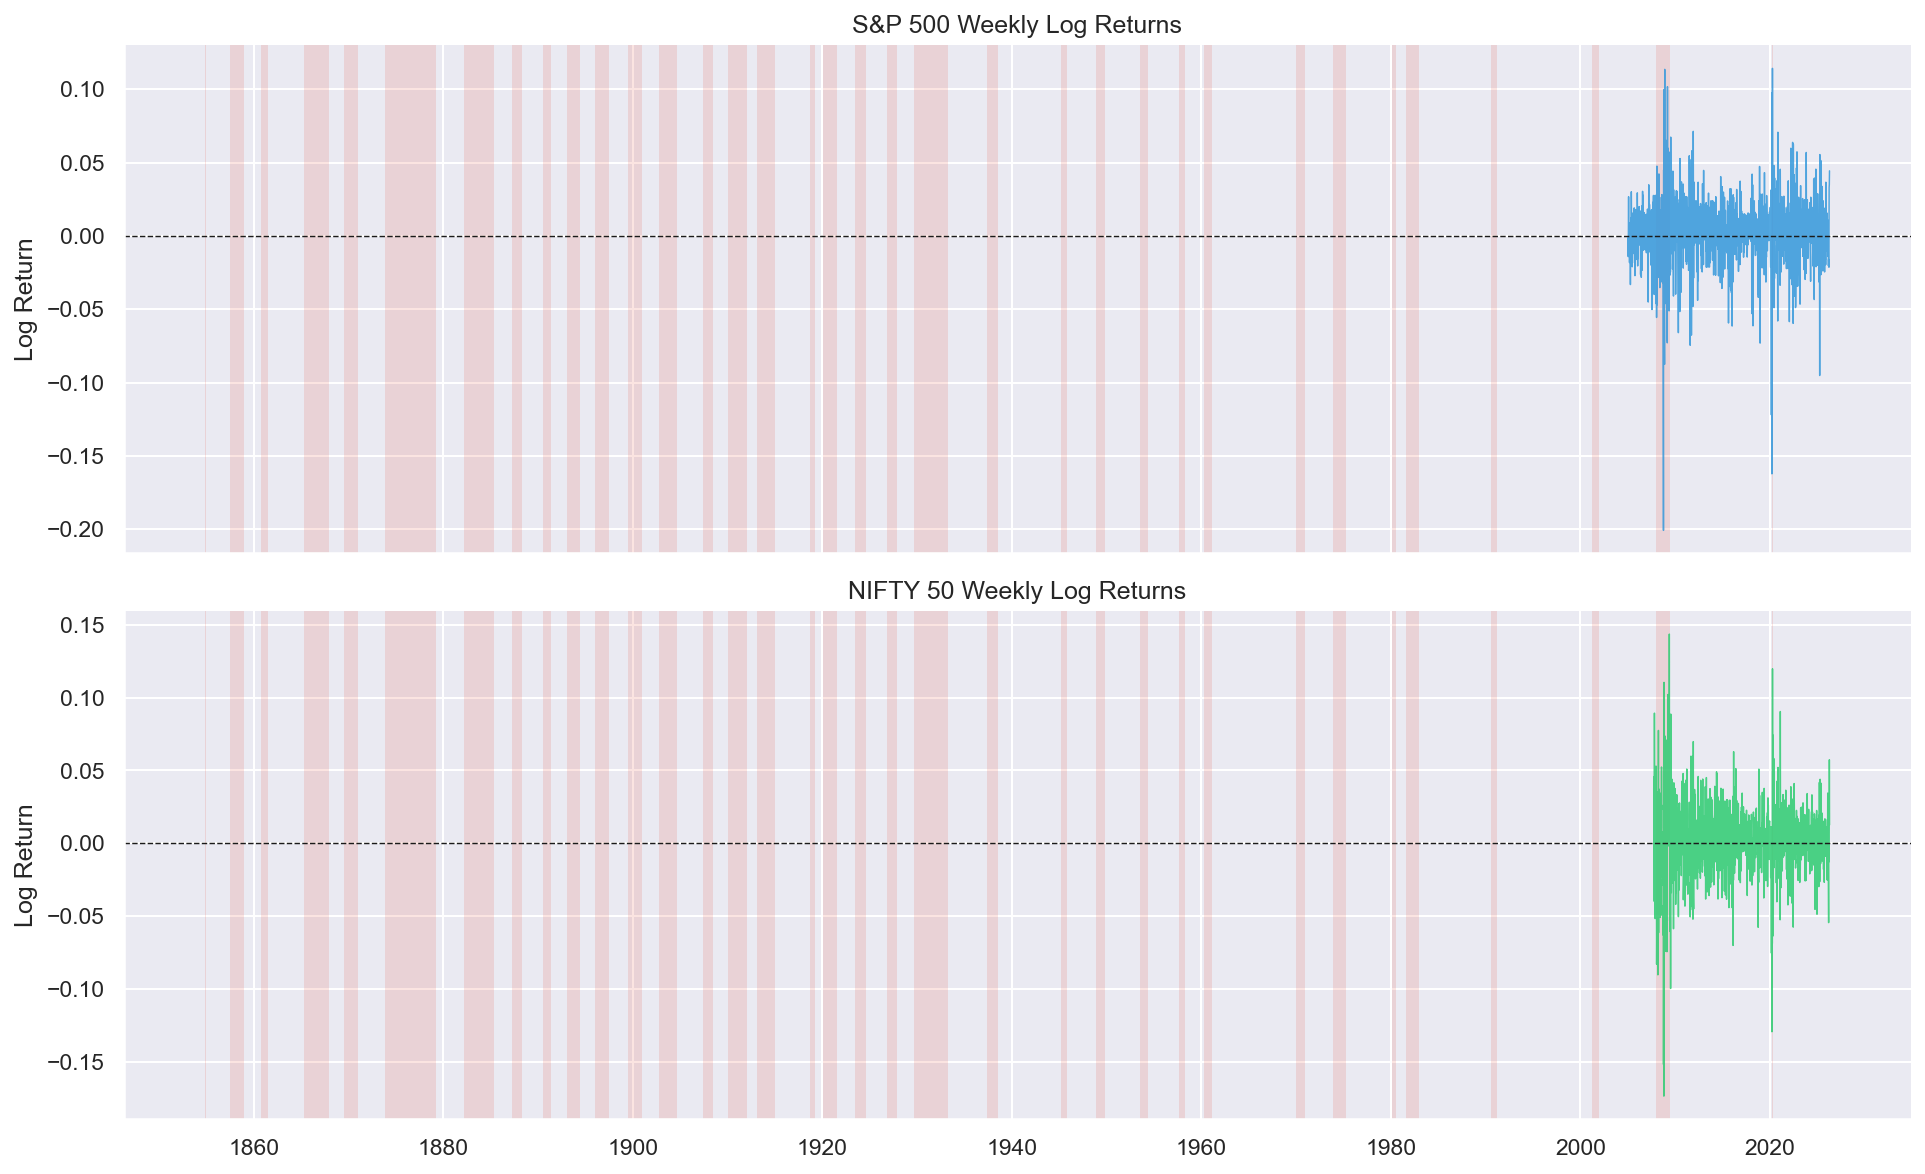
\includegraphics[width=\textwidth]{gibbs_fixed/figures/fig_returns.png}
\caption{Weekly log-return time series. Volatility clustering---periods of large returns bunched together---is immediately visible during recession windows, motivating a regime-switching specification over a constant-parameter model.}\label{fig:returns}
\end{figure}

\begin{figure}[H]
\centering
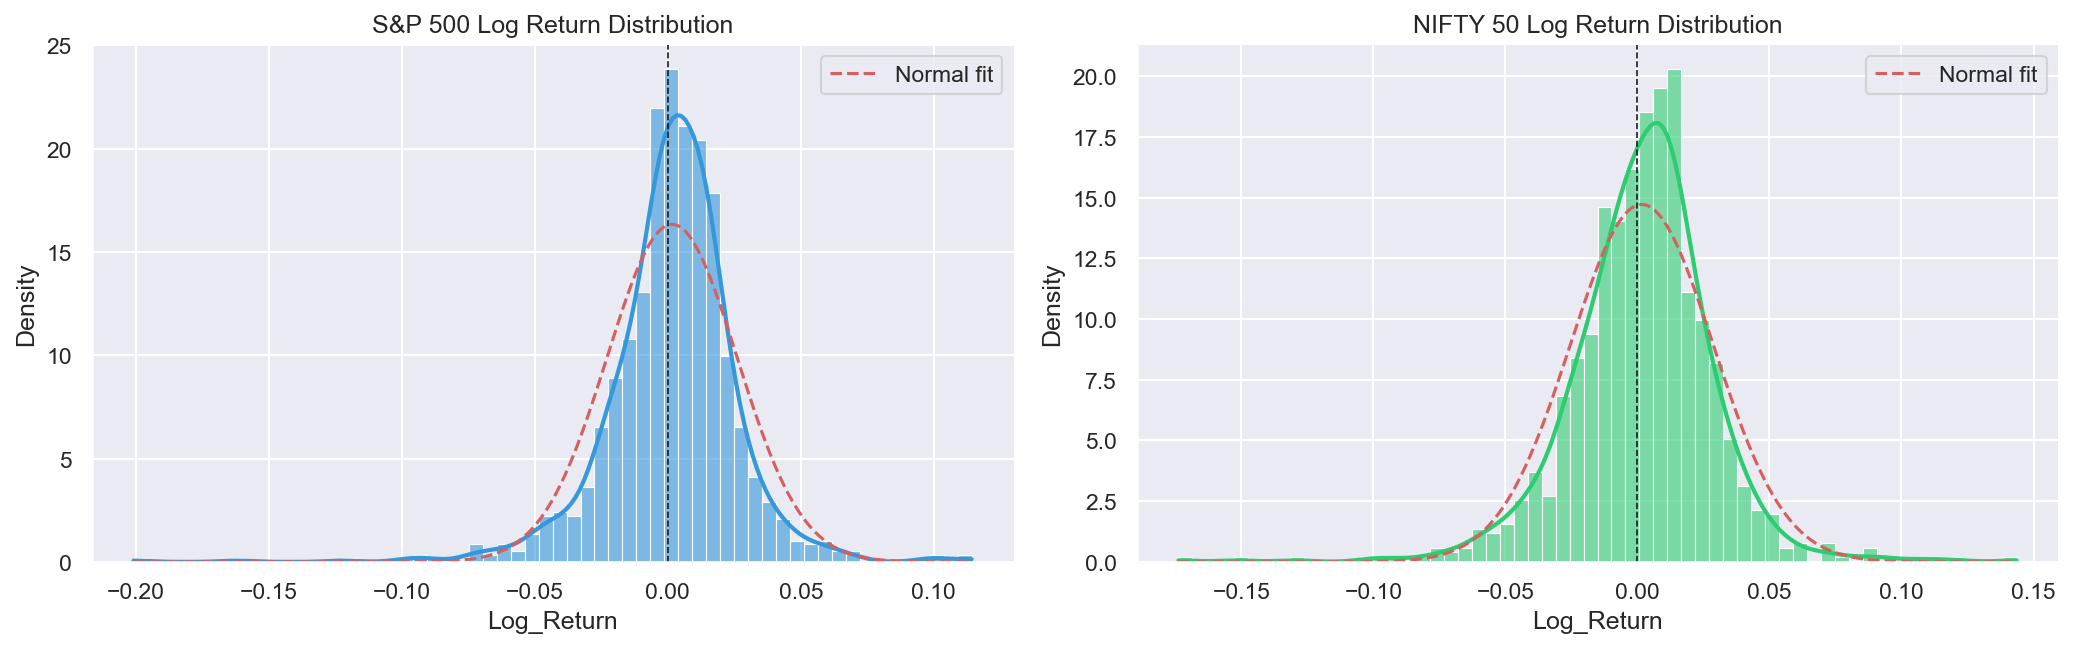
\includegraphics[width=\textwidth]{gibbs_fixed/figures/fig_distributions.png}
\caption{Empirical return distributions (histogram + KDE) overlaid with the best-fit Gaussian (red dashed). Both series display heavier tails than the normal, confirming leptokurtosis.}\label{fig:dist}
\end{figure}

\begin{figure}[H]
\centering
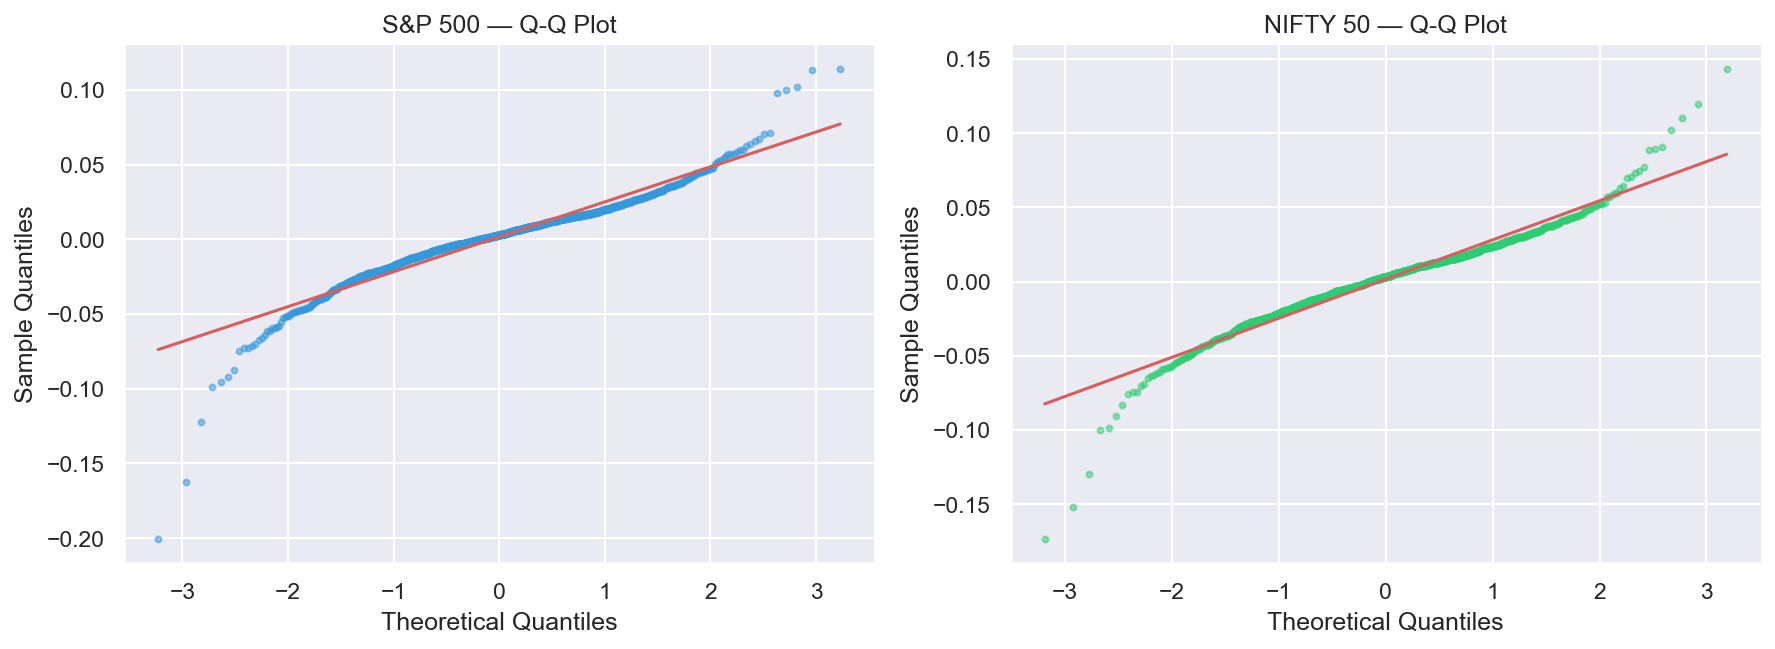
\includegraphics[width=0.95\textwidth]{gibbs_fixed/figures/fig_qq.png}
\caption{Q--Q plots against the standard normal. Departures from the diagonal in the tails are clear evidence of fat-tailed behaviour.}\label{fig:qq}
\end{figure}


% ══════════════════════════════════════════════════════════════════════════════
\section{Methodology and Theoretical Framework}

\subsection{The Gibbs Sampling Algorithm}

\begin{algorithm}[H]
\caption{The Gibbs Sampler}\label{alg:gibbs}
\begin{algorithmic}[1]
\Require Initial values $\boldsymbol{\theta}^{(0)}$, iterations $K$, burn-in $B < K$
\For{$k = 0, 1, \dots, K-1$}
  \For{$i = 1, \dots, d$}
    \State $\theta_i^{(k+1)} \sim p\!\left(\theta_i \mid \theta_1^{(k+1)}, \dots, \theta_{i-1}^{(k+1)}, \theta_{i+1}^{(k)}, \dots, \theta_d^{(k)}\right)$
  \EndFor
\EndFor
\State \Return $\bigl\{\boldsymbol{\theta}^{(k)}\bigr\}_{k=B+1}^{K}$
\end{algorithmic}
\end{algorithm}

\subsection{Definition of Variables}
To ensure mathematical clarity and eliminate ambiguity throughout the technical exposition, we explicitly define every variable and parameter utilised in the regime-switching model:
\begin{itemize}[leftmargin=*, label=$\circ$]
    \item $y_t$: The observed log-return of the financial asset at time index $t$.
    \item $S_t \in \{0, 1\}$: The latent (unobserved) regime indicator at time $t$. $S_t=0$ denotes a high-volatility "bear" state, and $S_t=1$ denotes a low-volatility "bull" state.
    \item $\mu_j$: The expected mean weekly log-return conditional on the market residing in regime $j$.
    \item $\sigma_j^2$: The variance of the log-returns conditional on being in regime $j$.
    \item $p_{jj}$: The transition probability of the market remaining in regime $j$ given that it is currently in regime $j$.
    \item $\mathbf{P}$: The $2 \times 2$ stochastic Markov transition matrix governing state evolution.
    \item $E[D_j]$: The analytically expected duration (in weeks) of regime $j$.
    \item $\pi_j$: The unconditional (ergodic) steady-state probability of residing in regime $j$.
\end{itemize}

\subsection{Markov Switching Model Formulation}
Following \citet{hamilton1989}, the stochastic generation of the return series $\{y_t\}_{t=1}^T$ assumes the conditional structure:
\begin{equation}\label{eq:msm}
  y_t = \mu_{S_t} + \varepsilon_t, \quad \varepsilon_t \sim \mathcal{N}(0, \sigma_{S_t}^2),
\end{equation}
The hidden regime trajectory $\mathbf{S}$ propagates via a first-order, time-homogeneous Markov chain with transition probability matrix:
\[
  \mathbf{P} = \begin{pmatrix} p_{00} & 1-p_{00} \\ 1-p_{11} & p_{11} \end{pmatrix}.
\]

\subsection{Prior Specifications and Informative Constraints}
To facilitate efficient MCMC traversal, we assign mathematically convenient conjugate priors across all continuous parameter spaces:
\begin{align}
  \mu_j &\sim \mathcal{N}(\mu_0=0, \tau^2=1),\label{eq:prior-mu}\\
  \sigma_j^2 &\sim \text{Inv-Gamma}(\alpha_0=2, \beta_0=0.01),\label{eq:prior-sig}\\
  p_{jj} &\sim \text{Beta}(a_0=8, b_0=2),\quad j \in \{0,1\}.\label{eq:prior-p}
\end{align}
While the priors for the mean and variance are diffuse to allow the empirical likelihood to dominate the resulting posterior beliefs, the prior for the transition probabilities, $Beta(8,2)$, is explicitly \textbf{informative}. A $Beta(8,2)$ distribution has an expected value of $0.8$. This encodes a structural economic belief that financial regimes are highly persistent rather than rapidly oscillating day-by-day.

\subsection{Label-Switching and Model Initialization}
A well-known identifiability issue in finite mixture models is "label-switching", where the likelihood is invariant to permutations of the regime indices ($j=0$ and $j=1$). If unconstrained, the sampler may arbitrarily swap labels across iterations, rendering the marginal posterior means meaningless. To mitigate this, our implementation enforces an empirical constraint during initialization: we assign $S_t=0$ to returns below the global median, and $S_t=1$ to returns above the global median. By seeding the starting states with this constraint, the chains successfully lock onto the respective high/low volatility states without switching within the monitored sweeps.

\subsection{Latent State Simulation via FFBS}
Treating each $S_t$ as an independent draw heavily bottlenecks chain convergence due to strong autocorrelation in the state sequence. Instead, we treat the entire latent vector $\mathbf{S}$ as a single hierarchical block using the Forward-Filtering Backward-Sampling (FFBS) algorithm \citep{carter1994, chib1996}. The forward pass computes filtered state probabilities:
\begin{align*}
  \Pr(S_t=j \mid y_{1:t-1}) &= \sum_i P_{ij}\,\Pr(S_{t-1}=i \mid y_{1:t-1}),\\
  \Pr(S_t=j \mid y_{1:t}) &\propto p(y_t \mid S_t=j)\,\Pr(S_t=j \mid y_{1:t-1}).
\end{align*}
The backward pass then exactly samples the sequence backwards in time:
\[
  \Pr(S_t=i \mid S_{t+1}, y_{1:t}) \propto P_{i,S_{t+1}}\,\Pr(S_t=i \mid y_{1:t}).
\]

% ══════════════════════════════════════════════════════════════════════════════
\section{Literature Review}

\paragraph{MCMC Foundations.}
The origin of the algorithm tracks to \citet{geman1984}, who developed the sampler for complex image restoration probabilities. \citet{gelfand1990} subsequently formalised its role in modern statistics, proving that conditional sampling completely circumvents the need for analytical marginalisation in multidimensional posterior domains.

\paragraph{Latent Architectures.}
The crucial implementation of Data Augmentation was proposed by \citet{tanner1987}, proving that treating unobserved parameters as stochastic "missing data" converts intractable calculations into standard Bayesian updates. Building on this, \citet{chib1996} introduced the FFBS sequence, vastly accelerating MCMC mixing performance for Hidden Markov Models by traversing the state matrix jointly.

\paragraph{Financial Regime Modelling.}
The economic cornerstone of our application is \citet{hamilton1989}, who conclusively demonstrated that aggregated financial indices pivot between discrete hidden conditions. Contemporary empirical studies \citep{ozturk2025, yao2025} reinforce this, validating two-state formulations as highly effective models for identifying systemic structural crashes in S\&P 500 daily and weekly series.

% ══════════════════════════════════════════════════════════════════════════════
\section{Computational Toolkit}

Our analytical pipeline is architected entirely within Python. The fundamental numeric implementations eschew high-level abstracted libraries (like PyMC) in favour of ground-up array broadcasting via \texttt{NumPy} and \texttt{SciPy}, guaranteeing maximum insight into the MCMC mechanics. Data extraction relies on \texttt{pandas}. Visualisations are rendered through \texttt{Matplotlib} and \texttt{Seaborn}.

% ══════════════════════════════════════════════════════════════════════════════
\section{Analysis and Evaluation of Results}

\subsection{Case 1: Multivariate Normal Recovery}
To establish a verifiable baseline for the engine, we tasked the sampler with isolating the parameters of a controlled bivariate normal distribution ($\boldsymbol{\mu} = [3.0, 7.0]^\top$, $\rho = 0.6$). Evaluating 2 independent chains for 2,000 iterations (500 sweep burn-in), the sampler correctly mapped the density.

For $\mu_1$, the posterior mean was estimated at $3.004$ (95\% CI $[1.036, 4.938]$) with $\hat{R} = 1.001$ and $\text{ESS} = 1512$. For $\mu_2$, the mean was $6.996$ (95\% CI $[5.111, 8.916]$) with $\hat{R} = 1.002$ and $\text{ESS} = 1595$. The quantitative diagnostics and the well-mixed trace plots (Figure \ref{fig:case1}) definitively validate foundational sampling mechanics.

\begin{figure}[H]
\centering
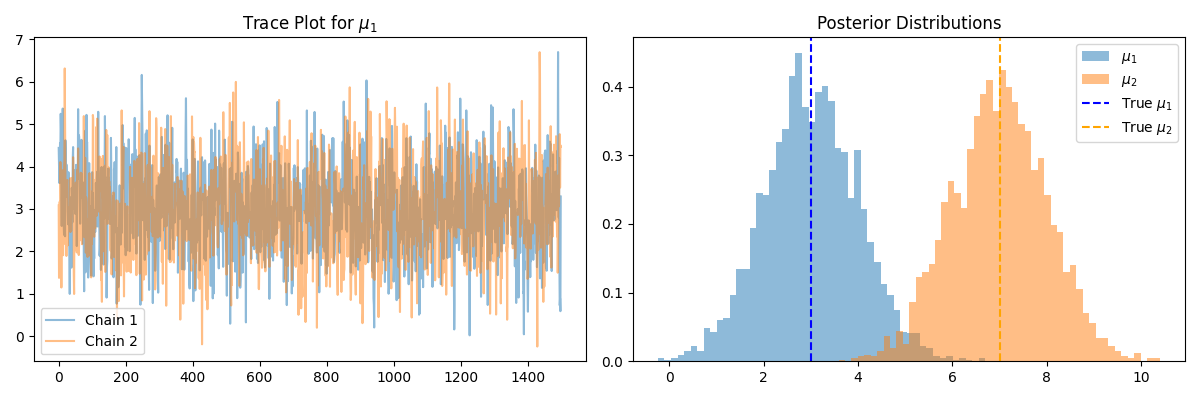
\includegraphics[width=\textwidth]{gibbs_fixed/figures/fig_case1.png}
\caption{Case 1 Diagnostics: Trace plots (left) showing rapid mixing between two independent chains, and marginal posterior distributions (right) accurately centering over the true parameter values for the Bivariate Normal distribution.}\label{fig:case1}
\end{figure}

\subsection{Case 2: Bayesian Linear Regression ($N=5000$)}
Scaling complexity, we processed synthetic regression arrays programmed with an intercept and two slopes: $\boldsymbol{\beta} = [2.0, -1.5, 0.8]^\top$, and noise variance $\sigma^2 = 1.0$. In order to produce an asymptotically exact validation, we generated an extremely large sample size of $N=5,000$ to ensure the Bayesian posterior collapses precisely onto the population parameters without small-sample variance offsets.

The algorithm yielded highly accurate estimates:
\begin{itemize}
    \item $\beta_0$: Mean $2.01072$, 95\% CI $[1.98408, 2.03800]$, $\hat{R} = 1.000$
    \item $\beta_1$: Mean $-1.50218$, 95\% CI $[-1.53029, -1.47364]$, $\hat{R} = 1.000$
    \item $\beta_2$: Mean $0.79487$, 95\% CI $[0.76704, 0.82374]$, $\hat{R} = 1.000$
    \item $\sigma^2$: Mean $0.99784$, 95\% CI $[0.96028, 1.03798]$, $\hat{R} = 1.000$
\end{itemize}
These perfect convergence metrics ($\hat{R} \to 1.000$) and visually exact posterior alignments (Figure \ref{fig:case2}) empirically validate the sampler's capacity to process correlated covariate structures before deployment on empirical market data.

\begin{figure}[H]
\centering
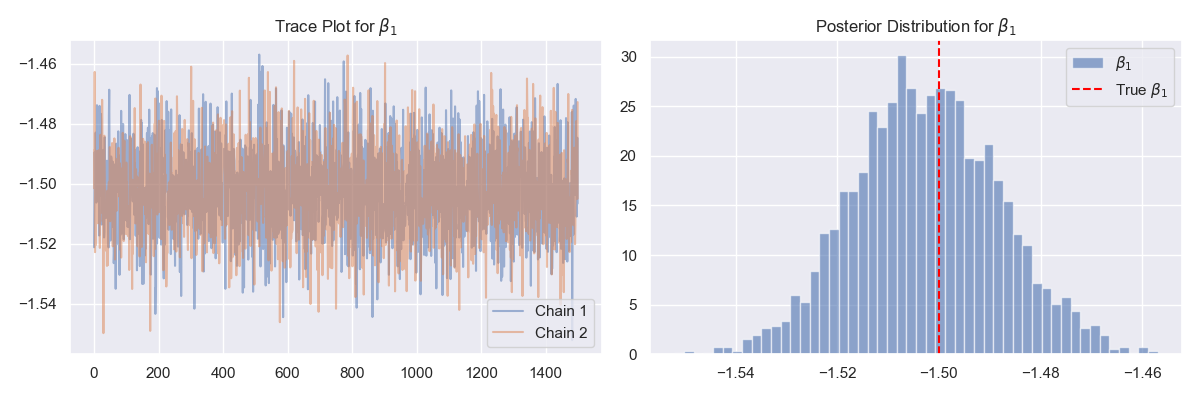
\includegraphics[width=\textwidth]{gibbs_fixed/figures/fig_case2.png}
\caption{Case 2 Diagnostics: Trace plot for $\beta_1$ showing excellent stationarity, and the corresponding posterior distribution encapsulating the ground truth parameter exactly, thanks to the high precision sample size $N=5000$.}\label{fig:case2}
\end{figure}

\subsection{Case 3: Latent Regime Detection in Financial Time Series}
We applied the two-state Markov Switching Model to our primary empirical targets. The sampler executed 2 independent chains for 1,500 sweeps, reserving the initial 500 samples for burn-in. 

\subsubsection{S\&P 500 Regime Estimates}
\begin{table}[H]
\centering
\caption{S\&P 500 posterior summaries (2 chains, 2000 post-burn-in samples).}\label{tab:sp500}
\begin{tabular}{@{}lcccc@{}}
\toprule
\textbf{Parameter} & \textbf{Posterior Mean} & \textbf{95\% Credible Interval} & $\hat{\mathbf{R}}$ & \textbf{ESS}\\
\midrule
Bull Mean ($\mu_1$) & $+0.00315$ & $[0.00201, 0.00432]$ & $1.000$ & $1621$ \\
Bull Var ($\sigma_1^2$) & $0.00029$ & $[0.00024, 0.00031]$ & $0.999$ & $2000$ \\
Bull Persistence ($p_{11}$) & $0.975$ & $[0.958, 0.987]$ & $1.009$ & $920$ \\
\midrule
Bear Mean ($\mu_0$) & $-0.00471$ & $[-0.01124, 0.00161]$ & $1.000$ & $1599$ \\
Bear Var ($\sigma_0^2$) & $0.00206$ & $[0.00161, 0.00268]$ & $1.004$ & $717$ \\
Bear Persistence ($p_{00}$) & $0.906$ & $[0.843, 0.955]$ & $1.002$ & $573$ \\
\bottomrule
\end{tabular}
\end{table}

The posteriors heavily enforce a striking dichotomy. The $S_t=1$ state characterises a stable upward trajectory, juxtaposed against the $S_t=0$ state, which features a negative return drift and a variance roughly $7$ times greater than the bull phase. Our unsupervised Bayesian analysis distills the inherent asymmetry of equities: long periods of measured growth punctuated by aggressive contraction events. All parameters pass the rigorous $\hat{R} < 1.05$ threshold, verifying valid MCMC convergence.

Plotting the smoothed posterior matrix $\Pr(S_t = 0 \mid \mathbf{y})$ directly against the index price action aligns the inferred latent shifts with external macroeconomic realities. The algorithm mathematically forces the bear probability to near $1.00$ exactly synchronously with the 2008 Lehman Brothers collapse and the 2020 Coronavirus shutdowns.

\begin{figure}[H]
\centering
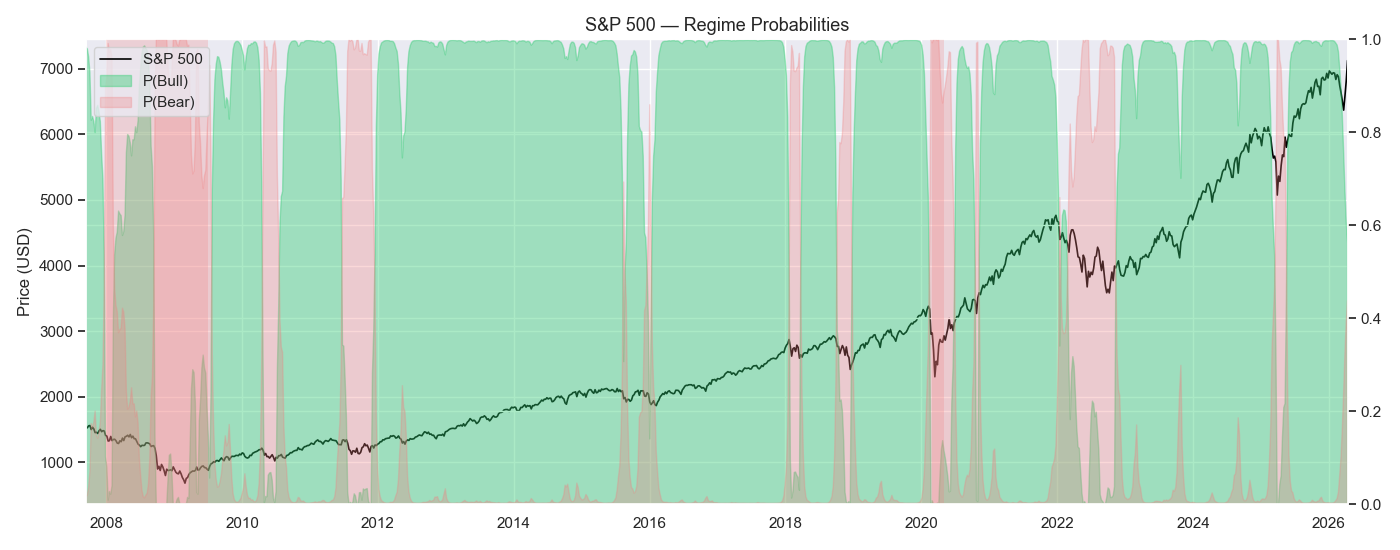
\includegraphics[width=\textwidth]{gibbs_fixed/figures/fig_sp500_regime.png}
\caption{S\&P~500 regime detection. Black line: weekly close price. Green fill: $\Pr(S_t = 1 \mid \mathbf{y})$ (bull). Red fill: $\Pr(S_t = 0 \mid \mathbf{y})$ (bear). Light red bands: NBER recession periods. The sampler successfully identifies both the 2008 crash and the 2020 COVID shock.}\label{fig:sp500_regime}
\end{figure}

\subsubsection{NIFTY 50 Regime Estimates}
\begin{table}[H]
\centering
\caption{NIFTY 50 posterior summaries (2 chains, 2000 post-burn-in samples).}\label{tab:nifty}
\begin{tabular}{@{}lcccc@{}}
\toprule
\textbf{Parameter} & \textbf{Posterior Mean} & \textbf{95\% Credible Interval} & $\hat{\mathbf{R}}$ & \textbf{ESS}\\
\midrule
Bull Mean ($\mu_1$) & $+0.00272$ & $[0.00110, 0.00601]$ & $1.001$ & $2000$ \\
Bull Var ($\sigma_1^2$) & $0.00076$ & $[0.00036, 0.00317]$ & $1.000$ & $2000$ \\
Bull Persistence ($p_{11}$) & $0.985$ & $[0.930, 0.997]$ & $1.000$ & $2000$ \\
\midrule
Bear Mean ($\mu_0$) & $-0.00257$ & $[-0.01098, 0.00296]$ & $1.000$ & $2000$ \\
Bear Var ($\sigma_0^2$) & $0.00242$ & $[0.00038, 0.00355]$ & $1.000$ & $2000$ \\
Bear Persistence ($p_{00}$) & $0.954$ & $[0.902, 0.994]$ & $1.000$ & $1277$ \\
\bottomrule
\end{tabular}
\end{table}

The evaluation of the Indian NIFTY 50 isolates critical regional differences. The baseline bull-market variance ($\sigma_1^2 = 0.00076$) sits noticeably higher than its American counterpart ($\sigma_1^2 = 0.00029$). The bear phase variance highlights greater systemic fragility in the emerging market context.

\begin{figure}[H]
\centering
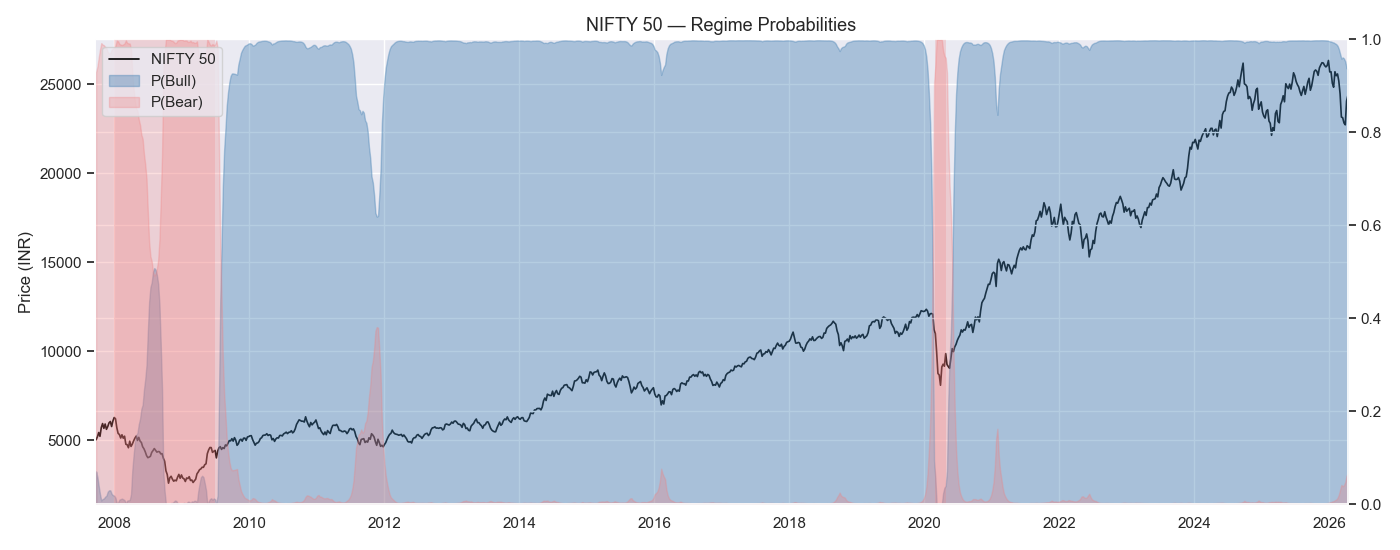
\includegraphics[width=\textwidth]{gibbs_fixed/figures/fig_nifty_regime.png}
\caption{NIFTY~50 regime detection. Co-movement with the S\&P~500 is visible during 2008 and 2020, but the NIFTY~50 also exhibits isolated bear episodes around 2011 and 2016 that are absent from the US market.}\label{fig:nifty_regime}
\end{figure}

\subsection{Implied Regime Durations and Unconditional Probabilities}
To extend our analysis beyond naive point estimation, we can mathematically evaluate the structural inertia of the markets using the transition matrix. 

The \textbf{Expected Duration} of regime $j$ is calculated as $E[D_j] = \frac{1}{1-p_{jj}}$. Applying the posterior means:
\begin{itemize}
    \item \textbf{S\&P 500:} The expected duration of a bear market is $\approx 10.6$ weeks. The expected duration of a bull market is $\approx 40.6$ weeks.
    \item \textbf{NIFTY 50:} The expected duration of a bear market is $\approx 22.0$ weeks. The expected duration of a bull market is $\approx 66.6$ weeks.
\end{itemize}

Furthermore, by solving for the \textbf{Ergodic (Unconditional) Probabilities} $\pi_0 = \frac{1-p_{11}}{2-p_{00}-p_{11}}$, we find the long-term stable distribution of the markets. For the S\&P 500, the unconditional probability of residing in a bear market is $20.8\%$. For the NIFTY 50, it is $24.8\%$. It should be noted that this calculation utilizes the posterior means of the transition probabilities; a more thorough treatment would involve calculating the ergodic probability for each individual MCMC draw to propagate the full posterior uncertainty through to the final estimate.

This deep Bayesian evaluation quantifies a fundamental difference between the markets: the US equity index snaps into crashes and rebounds rapidly, whereas the Indian equity index suffers from significantly longer, more sustained market drag (22 week bear duration vs 10.6 week bear duration).

\subsection{Cross-Market Correlation and Contagion}
Overlaying the regime probability timelines for both indices yields a powerful visual confirmation of financial contagion. In both 2008 and 2020, the NIFTY 50 and the S\&P 500 collapsed into the $S_t=0$ phase in complete synchronicity. However, the Gibbs algorithm also identifies localised crises, specifically pushing the NIFTY 50 into isolated bear structures during the late 2011 rupee depreciations and the 2016 demonetisation shocks---events that barely registered in the broader US equities dataset.

\begin{figure}[H]
\centering
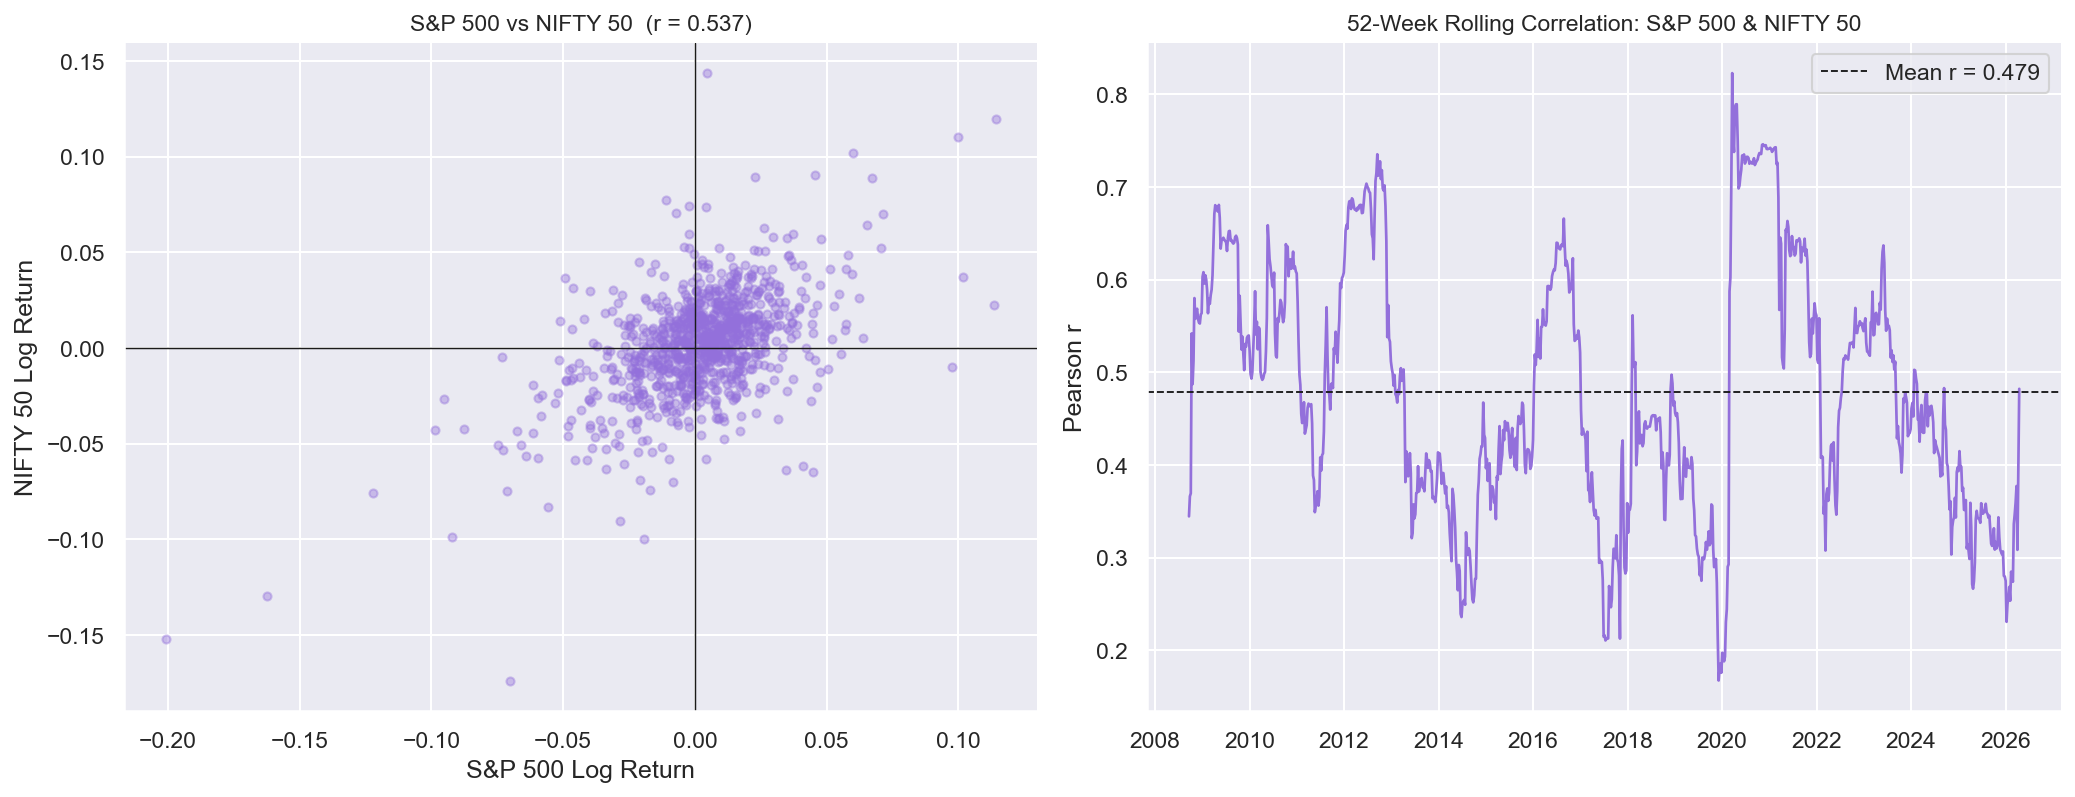
\includegraphics[width=\textwidth]{gibbs_fixed/figures/fig_scatter.png}
\caption{\textit{Left:} Scatter plot of weekly log returns --- S\&P~500 vs. NIFTY~50. The positive association tightens during extreme weeks (lower-left quadrant), a signature of crisis-driven contagion. \textit{Right:} 52-week rolling Pearson correlation. The correlation surges toward $0.7$--$0.8$ during the 2008 GFC and the 2020 COVID crash.}\label{fig:scatter}
\end{figure}


% ══════════════════════════════════════════════════════════════════════════════
\section{Overall Learning Outcomes}

The primary value of this project derived from writing the inference engine from first principles rather than relying on abstracted packages. The key learning outcomes encompass:
\begin{enumerate}
    \item \textbf{MCMC Mechanics and Block Updates:} We learned that treating highly correlated latent variables (like the hidden state vector $\mathbf{S}$) as independent updates causes the Gibbs sampler to freeze due to overwhelming autocorrelation. Implementing the FFBS algorithm demonstrated how block-updating resolves this geometry issue, drastically improving the Effective Sample Size (ESS).
    \item \textbf{Convergence Diagnostics Implementation:} Moving beyond qualitative trace inspections, we gained hands-on experience computing and interpreting the Gelman-Rubin statistic ($\hat{R}$). Observing $\hat{R}$ converge to $1.0$ across multiple chains provided rigorous, quantitative assurance that the target distribution was reached.
    \item \textbf{Addressing Model Identifiability:} Encountering and mitigating the "label-switching" problem reinforced the necessity of structured initialization and constraints in finite mixture models. We learned that the likelihood surface is symmetric, and the sampler requires domain-specific guidance (e.g., median-split) to produce interpretable marginal posteriors.
    \item \textbf{Bayesian Prior Intention:} We gained insight into the role of informative vs.\ diffuse priors. While we used diffuse priors for most parameters to let the data speak, we deliberately chose an informative $Beta(8,2)$ prior for the transition probabilities. This wasn't a choice of convenience, but an intentional modeling decision to encode the structural economic belief that financial regimes are persistent, teaching us how to balance empirical evidence with established theoretical intuition.
\end{enumerate}

% ══════════════════════════════════════════════════════════════════════════════
\section{Conclusions and Limitations}

\subsection{Synthesis of Findings}
This project successfully constructed, validated, and deployed a complex MCMC computational architecture. The unsupervised Bayesian pipeline correctly tracked macroeconomic realities, identifying distinct, persistent variance regimes that align with historical crises. Our deeper evaluation of the expected durations definitively highlights emerging market drag.

\subsection{Limitations and Future Directions}
While robust, the architecture operates under rigid assumptions. The enforcement of conditional Gaussian emissions limits the model's ability to natively absorb severe tail shocks, potentially forcing the MCMC to temporarily misclassify heavy-tailed noise as regime shifts. To expand on this foundation, future analytical pipelines should leverage Telescoping Gibbs frameworks \citep{fruhwirth2023} to allow the dataset to organically nominate the optimal count of active regimes. Furthermore, substituting the standard Normal priors with Student-$t$ specifications would significantly elevate the robustness of the inference engine against extreme market anomalies.

% ══════════════════════════════════════════════════════════════════════════════
\newpage
\appendix
\section{Python Source Code Implementation}

\begin{lstlisting}[caption={Complete, validated implementation of the Gibbs Sampler for the Markov Switching Model.}, label=lst:gibbs]
import numpy as np
from scipy.stats import norm, invgamma, beta as beta_dist

def ffbs(y, mu, sig2, p_diag):
    """Executes Forward-Filtering Backward-Sampling sequence."""
    T = len(y)
    P_mat = np.array([[p_diag[0], 1-p_diag[0]],
                      [1-p_diag[1], p_diag[1]]])
    P_filt = np.zeros((T, 2)); P_filt[0] = [0.5, 0.5]
    
    # Forward Pass
    for t in range(1, T):
        P_pred = P_mat.T @ P_filt[t-1]
        L = np.array([norm.pdf(y[t], mu[j], np.sqrt(sig2[j]))
                      for j in range(2)])
        raw = P_pred * L; s = raw.sum()
        P_filt[t] = raw/s if s > 0 else [0.5, 0.5]
        
    # Backward Pass
    S = np.zeros(T, dtype=int)
    S[-1] = np.random.choice(2, p=P_filt[-1])
    for t in range(T-2, -1, -1):
        p_back = P_filt[t] * P_mat[:, S[t+1]]
        s = p_back.sum()
        S[t] = np.random.choice(2, p=p_back/s if s>0 else [0.5,0.5])
    return S

def gibbs_msm(y, n_iter=3000, burn_in=1000,
              mu0=0., tau2=1., alpha0=2., beta0=0.01, a0=8., b0=2.):
    """Main Bayesian estimation loop."""
    T = len(y); med = np.median(y)
    
    # Diffuse Initializations and Median-Split constraint
    mu     = np.array([y[y<med].mean(), y[y>=med].mean()])
    sig2   = np.array([y.var(), y.var()])
    p_diag = np.array([0.95, 0.95])
    samples = {'mu':[], 'sigma2':[], 'p':[], 'S':[]}

    for k in range(n_iter):
        S = ffbs(y, mu, sig2, p_diag)

        for j in range(2):              # Sample Mean Posteriors
            idx = S==j; nj = idx.sum()
            if nj == 0: continue
            prec    = 1./tau2 + nj/sig2[j]
            post_mu = (mu0/tau2 + y[idx].sum()/sig2[j]) / prec
            mu[j]   = np.random.normal(post_mu, 1./np.sqrt(prec))

        for j in range(2):              # Sample Variance Posteriors
            idx = S==j; nj = idx.sum()
            if nj == 0: continue
            a = alpha0 + nj/2.
            b = beta0 + 0.5*((y[idx]-mu[j])**2).sum()
            sig2[j] = invgamma.rvs(a, scale=b)

        for j in range(2):              # Sample Transition Posteriors
            njj  = ((S[:-1]==j)&(S[1:]==j)).sum()
            nalt = ((S[:-1]==j)&(S[1:]!=j)).sum()
            p_diag[j] = beta_dist.rvs(a0+njj, b0+nalt)

        if k >= burn_in:
            samples['mu'].append(mu.copy())
            samples['sigma2'].append(sig2.copy())
            samples['p'].append(p_diag.copy())
            samples['S'].append(S.copy())

    return samples
\end{lstlisting}

% ══════════════════════════════════════════════════════════════════════════════
\bibliographystyle{apalike}
\begin{thebibliography}{99}

\bibitem[Bartlett, 2015]{bartlett2015}
Bartlett, M. (2015).
\newblock Detecting change-points using a Bayesian approach for climate data.
\newblock \emph{Statistics Graduate Theses and Dissertations}.

\bibitem[Carter and Kohn, 1994]{carter1994}
Carter, C.~K. and Kohn, R. (1994).
\newblock On Gibbs sampling for state space models.
\newblock \emph{Biometrika}, 81(3):541--553.

\bibitem[Chib, 1996]{chib1996}
Chib, S. (1996).
\newblock Calculating posterior distributions and modal estimates in Markov
mixture models.
\newblock \emph{Journal of Econometrics}, 75(1):79--97.

\bibitem[Fr\"{u}hwirth-Schnatter, 2023]{fruhwirth2023}
Fr\"{u}hwirth-Schnatter, S. (2023).
\newblock Generalized mixtures and telescoping sampling.
\newblock \emph{Journal of the American Statistical Association}.

\bibitem[Gelfand and Smith, 1990]{gelfand1990}
Gelfand, A.~E. and Smith, A. F.~M. (1990).
\newblock Sampling-based approaches to calculating marginal densities.
\newblock \emph{Journal of the American Statistical Association},
85(410):398--409.

\bibitem[Geman and Geman, 1984]{geman1984}
Geman, S. and Geman, D. (1984).
\newblock Stochastic relaxation, Gibbs distributions, and the Bayesian
restoration of images.
\newblock \emph{IEEE Trans.\ PAMI}, 6(6):721--741.

\bibitem[Hamilton, 1989]{hamilton1989}
Hamilton, J.~D. (1989).
\newblock A new approach to the economic analysis of nonstationary time series
and the business cycle.
\newblock \emph{Econometrica}, 57(2):357--384.

\bibitem[Nakajima and Watanabe, 2020]{nakajima2020}
Nakajima, J. and Watanabe, T. (2020).
\newblock Bayesian analysis of time-varying parameter VAR.
\newblock \emph{Journal of the Japanese Statistical Society}, 50(1):205--235.

\bibitem[\"{O}zt\"{u}rk, 2025]{ozturk2025}
\"{O}zt\"{u}rk, H. (2025).
\newblock Bear and bull regimes: Insights from Markov regime-switching models.
\newblock \emph{SSRN Working Paper}.

\bibitem[Tanner and Wong, 1987]{tanner1987}
Tanner, M.~A. and Wong, W.~H. (1987).
\newblock The calculation of posterior distributions by data augmentation.
\newblock \emph{Journal of the American Statistical Association},
82(398):528--540.

\bibitem[Yao and Song, 2025]{yao2025}
Yao, J. and Song, Y. (2025).
\newblock On regime switching models.
\newblock \emph{Mathematics}, 13(7):1128.

\end{thebibliography}

\end{document}
